% Standalone TikZ figure: Book Organization Roadmap
% For Chapter 1: Introduction - Section 1.5 Contributions and Organization
\documentclass[tikz,border=10pt]{standalone}
\usepackage{tikz}
\usepackage{amsmath}
\usetikzlibrary{arrows.meta, positioning, shapes.geometric, calc, fit, backgrounds}

\begin{document}
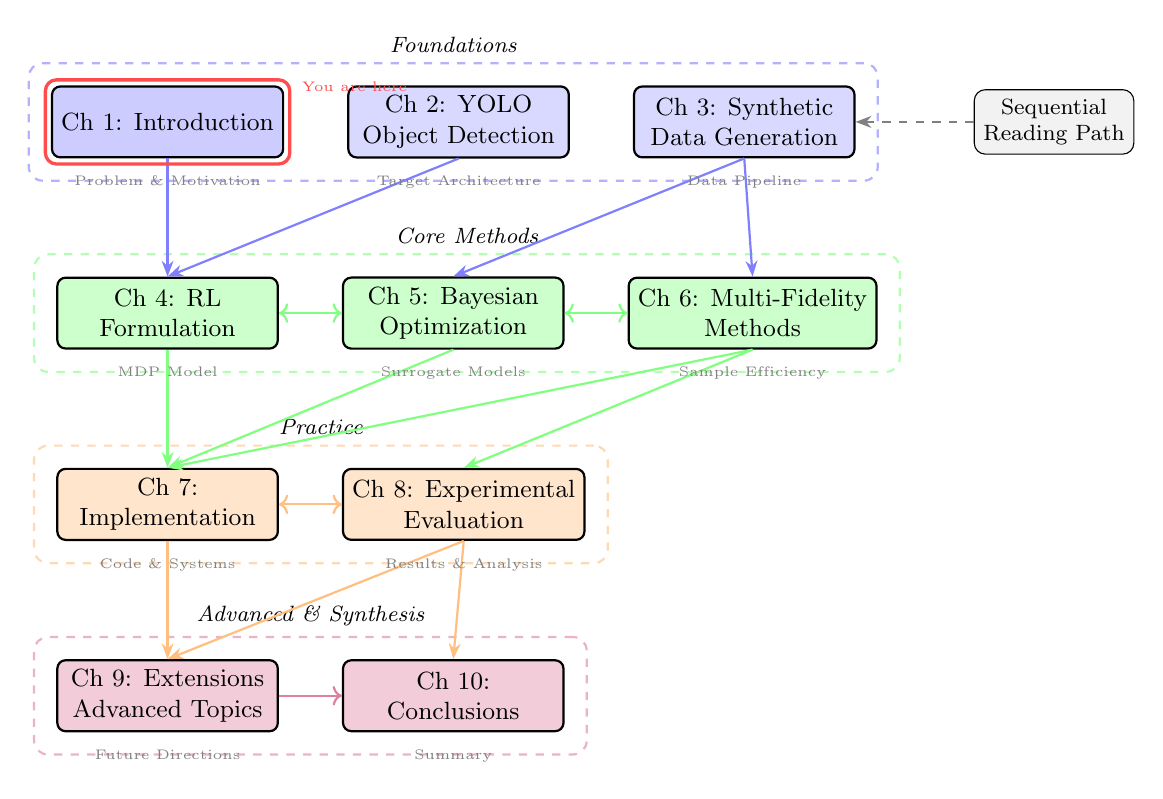
\begin{tikzpicture}[
    node distance=0.5cm and 0.8cm,
    every node/.style={font=\small},
    chapter/.style={rectangle, draw, thick, minimum width=2.8cm, minimum height=0.9cm, align=center, rounded corners=3pt, fill=#1},
    group/.style={draw, dashed, thick, rounded corners=5pt, inner sep=8pt, #1},
    arrow/.style={-{Stealth[length=2mm]}, thick, #1},
    title/.style={font=\bfseries\small},
    grouplabel/.style={font=\footnotesize\itshape, fill=white}
]

% Row 1: Foundations
\node[chapter=blue!20] (ch1) {Ch 1: Introduction};
\node[chapter=blue!15, right=of ch1] (ch2) {Ch 2: YOLO\\Object Detection};
\node[chapter=blue!15, right=of ch2] (ch3) {Ch 3: Synthetic\\Data Generation};

% Row 2: Core Methods
\node[chapter=green!20, below=1.5cm of ch1] (ch4) {Ch 4: RL\\Formulation};
\node[chapter=green!20, right=of ch4] (ch5) {Ch 5: Bayesian\\Optimization};
\node[chapter=green!20, right=of ch5] (ch6) {Ch 6: Multi-Fidelity\\Methods};

% Row 3: Practice
\node[chapter=orange!20, below=1.5cm of ch4] (ch7) {Ch 7:\\Implementation};
\node[chapter=orange!20, right=of ch7] (ch8) {Ch 8: Experimental\\Evaluation};

% Row 4: Advanced
\node[chapter=purple!20, below=1.5cm of ch7] (ch9) {Ch 9: Extensions\\Advanced Topics};
\node[chapter=purple!20, right=of ch9] (ch10) {Ch 10:\\Conclusions};

% Group boxes
\begin{scope}[on background layer]
\node[group=blue!30, fit=(ch1)(ch2)(ch3), label={[grouplabel]above:Foundations}] (g1) {};
\node[group=green!30, fit=(ch4)(ch5)(ch6), label={[grouplabel]above:Core Methods}] (g2) {};
\node[group=orange!30, fit=(ch7)(ch8), label={[grouplabel]above:Practice}] (g3) {};
\node[group=purple!30, fit=(ch9)(ch10), label={[grouplabel]above:Advanced \& Synthesis}] (g4) {};
\end{scope}

% Vertical flow arrows
\draw[arrow=blue!50] (ch1.south) -- (ch4.north);
\draw[arrow=blue!50] (ch2.south) -- (ch4.north);
\draw[arrow=blue!50] (ch3.south) -- (ch5.north);
\draw[arrow=blue!50] (ch3.south) -- (ch6.north);

% Horizontal dependencies within core methods
\draw[arrow=green!50, <->] (ch4) -- (ch5);
\draw[arrow=green!50, <->] (ch5) -- (ch6);

% Flow to practice
\draw[arrow=green!50] (ch4.south) -- (ch7.north);
\draw[arrow=green!50] (ch5.south) -- (ch7.north);
\draw[arrow=green!50] (ch6.south) -- (ch8.north);
\draw[arrow=green!50] (ch6.south) -- (ch7.north);

% Horizontal in practice
\draw[arrow=orange!50, <->] (ch7) -- (ch8);

% Flow to advanced
\draw[arrow=orange!50] (ch7.south) -- (ch9.north);
\draw[arrow=orange!50] (ch8.south) -- (ch9.north);
\draw[arrow=orange!50] (ch8.south) -- (ch10.north);
\draw[arrow=purple!50, ->] (ch9) -- (ch10);

% Reading path annotations
\node[draw, rounded corners, fill=gray!10, font=\footnotesize, align=center,
      right=1.5cm of ch3] (path1) {Sequential\\Reading Path};
\draw[arrow=gray, dashed] (path1.west) -- (ch3.east);

% Key concepts annotations
\node[font=\tiny, gray, below=0.1cm of ch1] {Problem \& Motivation};
\node[font=\tiny, gray, below=0.1cm of ch2] {Target Architecture};
\node[font=\tiny, gray, below=0.1cm of ch3] {Data Pipeline};
\node[font=\tiny, gray, below=0.1cm of ch4] {MDP Model};
\node[font=\tiny, gray, below=0.1cm of ch5] {Surrogate Models};
\node[font=\tiny, gray, below=0.1cm of ch6] {Sample Efficiency};
\node[font=\tiny, gray, below=0.1cm of ch7] {Code \& Systems};
\node[font=\tiny, gray, below=0.1cm of ch8] {Results \& Analysis};
\node[font=\tiny, gray, below=0.1cm of ch9] {Future Directions};
\node[font=\tiny, gray, below=0.1cm of ch10] {Summary};

% Current chapter indicator
\node[draw, very thick, red!70, rounded corners, fit=(ch1), inner sep=2pt] {};
\node[font=\tiny, red!70, above right=-0.2cm and 0.1cm of ch1] {You are here};

\end{tikzpicture}
\end{document}
